% This file was converted to LaTeX by Writer2LaTeX ver. 1.4
% see http://writer2latex.sourceforge.net for more info
\documentclass[a4paper]{article}
\usepackage[utf8]{inputenc}
\usepackage[T1]{fontenc}
\usepackage[ngerman]{babel}
\usepackage{amsmath}
\usepackage{amssymb,amsfonts,textcomp}
\usepackage{color}
\usepackage{array}
\usepackage{hhline}
\usepackage{hyperref}
\hypersetup{pdftex, colorlinks=true, linkcolor=blue, citecolor=blue, filecolor=blue, urlcolor=blue, pdftitle=}
\usepackage[pdftex]{graphicx}
% footnotes configuration
\makeatletter
\renewcommand\thefootnote{\arabic{footnote}}
\makeatother
% Text styles
\newcommand\textstyleAbsatzStandardschriftart[1]{#1}
\newcommand\textstyleFootnoteSymbol[1]{#1}
\newcommand\textstyleHyperlink[1]{\textcolor{blue}{#1}}
% Outline numbering
\setcounter{secnumdepth}{0}
% List styles
\newcommand\liststyleLi{%
\renewcommand\theenumi{\arabic{enumi}}
\renewcommand\theenumii{\arabic{enumii}}
\renewcommand\theenumiii{\arabic{enumiii}}
\renewcommand\theenumiv{\arabic{enumiv}}
\renewcommand\labelenumi{\theenumi.}
\renewcommand\labelenumii{\theenumii.}
\renewcommand\labelenumiii{\theenumiii.}
\renewcommand\labelenumiv{\theenumiv.}
}
\newcommand\liststyleLii{%
\renewcommand\labelitemi{•}
\renewcommand\labelitemii{◦}
\renewcommand\labelitemiii{${\blacksquare}$}
\renewcommand\labelitemiv{•}
}
\newcommand\liststyleLiii{%
\renewcommand\labelitemi{{\textbullet}}
\renewcommand\labelitemii{o}
\renewcommand\labelitemiii{${\blacksquare}$}
\renewcommand\labelitemiv{{\textbullet}}
}
\newcommand\liststyleLiv{%
\renewcommand\labelitemi{{\textbullet}}
\renewcommand\labelitemii{o}
\renewcommand\labelitemiii{${\blacksquare}$}
\renewcommand\labelitemiv{{\textbullet}}
}
% Page layout (geometry)
\setlength\voffset{-1in}
\setlength\hoffset{-1in}
\setlength\topmargin{2cm}
\setlength\oddsidemargin{3.5cm}
\setlength\textheight{22.706001cm}
\setlength\textwidth{15.500999cm}
\setlength\footskip{1.497cm}
\setlength\headheight{0.998cm}
\setlength\headsep{0.499cm}
% Footnote rule
\setlength{\skip\footins}{0.119cm}
\renewcommand\footnoterule{\vspace*{-0.018cm}\setlength\leftskip{0pt}\setlength\rightskip{0pt plus 1fil}\noindent\textcolor{black}{\rule{0.25\columnwidth}{0.018cm}}\vspace*{0.101cm}}
% Pages styles
\makeatletter
\newcommand\ps@Standard{
  \renewcommand\@oddhead{\sffamily INM - Potentielle Neuordnung des Informationsmanagements\hfill 29.05.15}
  \renewcommand\@evenhead{\@oddhead}
  \renewcommand\@oddfoot{\sffamily INM – SoSe 2015\hfill \hfill \thepage{} / ?}
  \renewcommand\@evenfoot{\@oddfoot}
  \renewcommand\thepage{\arabic{page}}
}
\makeatother
\pagestyle{Standard}
% Non-floating captions
\makeatletter
\newcommand\captionof[1]{\def\@captype{#1}\caption}
\makeatother
\title{}
\begin{document}
\setcounter{tocdepth}{10}
\renewcommand\contentsname{Inhaltsverzeichnis}
\tableofcontents
\section[2\ \ Ist{}-Situation der Hochschule Emden/Leer[2028?]hinsichtlich wichtiger Dimensionen]{2\ \ Ist-Situation der
Hochschule Emden/Leer[2028?]hinsichtlich wichtiger Dimensionen}
\subsection[2.1 Ziel]{\bfseries 2.1 Ziel}
{\sffamily\mdseries\color{black}
Mit Hilfe der Analyse der IST-Situation an der Hochschule Emden/Leer wird festgestellt in wieweit an der Hochschule
bereits ein Informationsmanagement besteht. Wenn dies nicht der Fall ist wird recherchiert, welche Informationen
bereits zentral gesammelt werden und welche Bereiche in das Projekt „\textbf{Potentielle Neuordnung des
Informationsmanagements einer kleineren Fachhochschule auf der Grundlage bestehender Lösungen an deutschen
Hochschulen“} mit einbezogen werden müssen.}


\bigskip

\subsection[2.2 Aufgaben]{\bfseries 2.2 Aufgaben}
{\sffamily\mdseries\color{black}
Wesentliche Fragestellungen, welche in diesem Kapitel gelöst werden sollen, sind auf der einen Seite, welche vorhandene
IT-Systeme bereits zentral Verwendung finden und auf der anderen Seite, wie Informationen bereits Repräsentiert werden.
In dieser Analyse wird Aufschluss darüber gegeben, ob ein Informationsmanagement bereits an der Hochschule betrieben
wird oder wie Informationen bereits zentral zur Verfügung gestellt werden. }

{\sffamily\mdseries\color{black}
Bei der Hochschule Emden-Leer handelt es sich um eine kleine Hochschule mit aktuell
\textstyleAbsatzStandardschriftart{4626} eingeschriebenen Studierenden. \ Den größten Anteil machen die 4303 Studenten
vor Ort aus.
\footnote{http://www.hs-emden-leer.de/fileadmin/user\_upload/Einrichtungen/ZDF/Studierende/JV\_Stud\_20142.pdf}\textstyleFootnoteSymbol{
}Es sind 396 Mitarbeiter beschäftigt, wobei 107 Professuren sind.
\footnote{https://www.hs-emden-leer.de/no\_cache/hochschule/zahlen-daten-fakten.html}}


\bigskip

{\sffamily\mdseries\color{black}
\textstyleFootnoteSymbol{Der wesentliche Bestandteil dieses Kapitels ist der Prozess der Sammlung, Selektion und Prüfung
von Fragestellung, welche die Grundlage für ein Experten Interview bilden. Dieses Interview wurde durch die
Studierenden Tina Koppermann, Marc Enders, der betreuenden Professorin Frau Prof. Dr. Krüger-Basener mit dem Leiter des
Hochschulzentrums Emden/Leer Herrn Günter Müller durchgeführt. }}


\bigskip

{\sffamily\mdseries\color{black}
Es wurde bei der Erstellung dieses Experten Interviews auf die Methodik des SPSS-Prinzips verstärkt reflektiert. Dem
SPSS-Prinzip nach Helfferich\footnote{\ Helfferich, Cornelia (2009): Die Qualität qualitativer Daten. Manual für die
Durchführung qualitativer Interviews. 3., überarbeitete Auflage. Wiesbaden: VS Verlag für Sozialwissenschaften / GWV
Fachverlage GmbH, Wiesbaden (SpringerLink : Bücher)} liegt folgendes Vorgehen zur Grunde:}


\bigskip

\liststyleLi
\begin{enumerate}
\item {\sffamily\color{black}
Sammeln}
\item {\sffamily\color{black}
Prüfen}
\item {\sffamily\color{black}
Selektieren}
\item {\sffamily\color{black}
Subsumieren}


\bigskip
\end{enumerate}
{\sffamily\mdseries\color{black}
Mit Hilfe von diesem Prinzip zur qualitativen Datenerhebung werden im ersten Schritt Fragen gesammelt. Diese konnten von
allen Kursteilnehmern in einem zur Verfügung gestellten Online-Dokument eingesehen und editiert werden. Bei der
Sammlung der Fragen wurden insgesamt 62 Fragestellungen zu unterschiedlichen Schwerpunkten aufgenommen.}

{\sffamily\mdseries\color{black}
Nach der erfolgten Sammlung aller Fragen folgte im zweiten Schritt die Prüfung der Fragen. Hierbei wurden Fragen, welche
offen gestellt wurden, aussortiert. Nach der erfolgreichen Prüfung der Fragen folgte im nächsten Schritt die Selektion
von diesen. Es wurden die Fragegestellungen entsprechend Themengebieten zugeordnet und zusammengestellt. Im letzten
Schritt, dem Subsumieren des SPSS-Prinzips, wurde für jedes Themengebiet eine Erzähl Aufforderung gefunden und der
Interviewleitfaden entsprechend diesen Erzähl Aufforderungen gegliedert. Mit Hilfe eines Farbcodes (siehe Abbildung
\ 2) wurden die Fragen entsprechend nach Erzähl Aufforderung, Checkliste, konkreter Frage und Aufrechterhaltungsfrage
farblich markiert und anschließend einsortiert. }

\begin{figure}
\centering
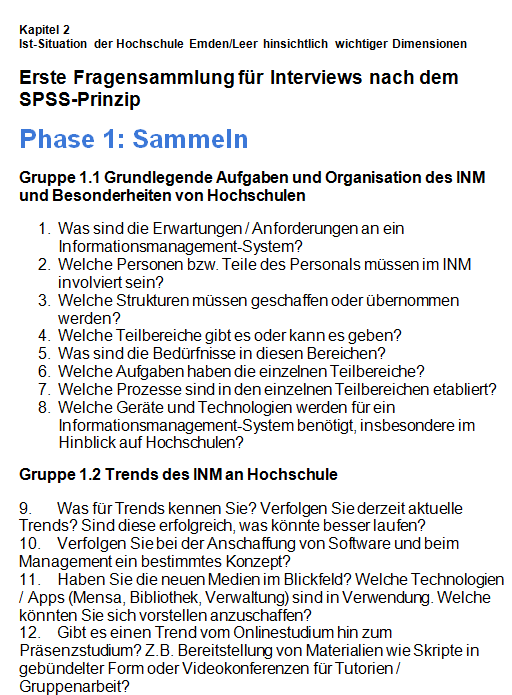
\includegraphics[width=8.585cm,height=11.652cm]{EntwurfKapitel2Gruppe220150528VW-img/EntwurfKapitel2Gruppe220150528VW-img001.png}
\caption[Exemplarischer Auszug aus Fragen Sammeln]{Exemplarischer Auszug aus Fragen Sammeln}

\end{figure}


\begin{figure}
\centering
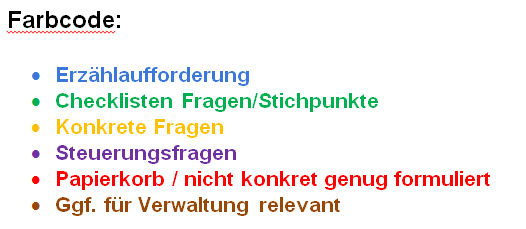
\includegraphics[width=9.546cm,height=3.868cm]{EntwurfKapitel2Gruppe220150528VW-img/EntwurfKapitel2Gruppe220150528VW-img002.png}
\caption[angewandter Farbcode für das SPSS{}-Prinzip]{angewandter Farbcode für das SPSS-Prinzip}

\end{figure}
{\sffamily\mdseries\color{black}
Diese Subsumierung wurde mit Hilfe des Anwendungsprogramms Microsoft Excel entsprechend visualisiert. Als Endergebnis
\ ist ein Interviewleitfaden entstanden, der in acht unterschiedliche Themenbereiche unterteilt wurde.}

\begin{figure}
\centering
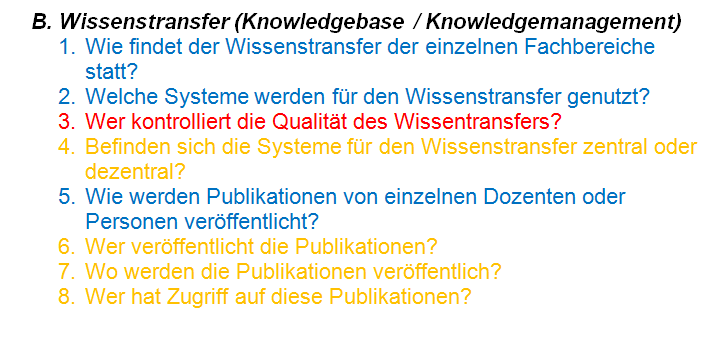
\includegraphics[width=11.575cm,height=5.269cm]{EntwurfKapitel2Gruppe220150528VW-img/EntwurfKapitel2Gruppe220150528VW-img003.png}
\caption[Sortierung der Fragen nach Fragentyp]{Sortierung der Fragen nach Fragentyp}

\end{figure}
{\sffamily\mdseries\color{black}
An dem festgelegtem Interviewtermin ist mit Hilfe von diesem Leitfaden das Experten Interview mit Herrn Günter Müller,
dem Leiter des Hochschulrechenzentrums an der Fachhochschule Emden/Leer, durchgeführt worden. Dieses Interview fand mit
der Online Video Plattform „Adobe Connect“ statt und wurde mit Zustimmung von Herrn Müller digital aufgezeichnet. Im
Anschluss an das Experten Interview wurde in der ersten Phase das Video auf wichtige inhaltliche Aspekte analysiert. }

\begin{figure}
\centering
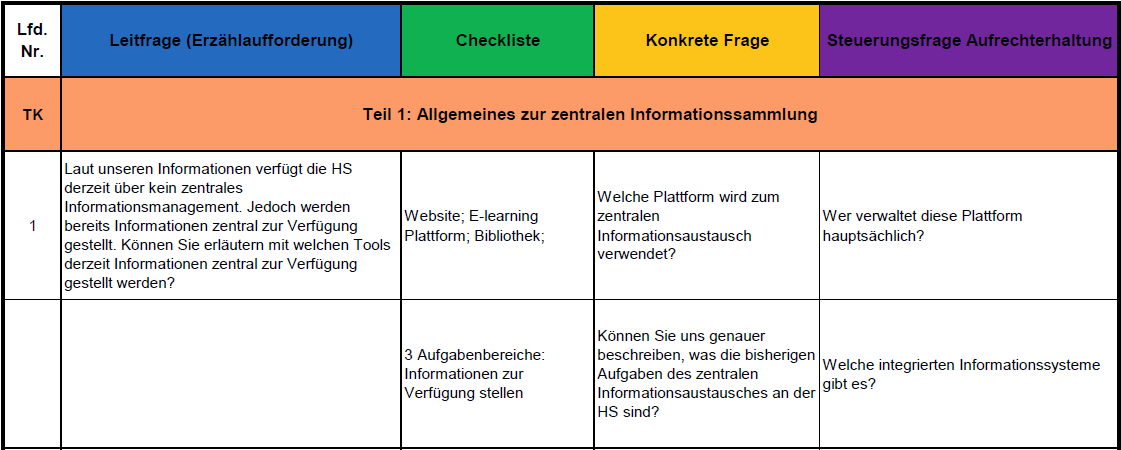
\includegraphics[width=15.501cm,height=6.223cm]{EntwurfKapitel2Gruppe220150528VW-img/EntwurfKapitel2Gruppe220150528VW-img004.png}
\caption[Exemplarischer Auszug des Interviewleitfadens]{Exemplarischer Auszug des Interviewleitfadens}

\end{figure}

\bigskip

{\sffamily\mdseries\color{black}
In der zweiten Phase wurde durch Transkription die digitale Aufzeichnung, mit Hilfe von der Applikation „Microsoft
Word“, überführt. Mit dem Ziel die im Interview genannten Informationen besser verarbeiten zu können. }


\bigskip

{\sffamily\mdseries\color{black}
In der darauffolgenden Phase wurden mit Hilfe des Tools „Xmind“ zu jedem Themenbereich Mindmaps generiert, um bei der
Recherche schneller auf Besonderheiten eingehen zu können.}


\bigskip

{\sffamily\mdseries\color{black}
Die Ergebnisse dieser IST-Analyse werden in den folgenden Kapiteln detaillierter beschrieben. }


\bigskip


\bigskip

\subsection[2.3 Zuständigkeiten]{\bfseries 2.3 Zuständigkeiten}
{\sffamily\mdseries\color{black}
In diesem Kapitel wird auf die Zuständigkeiten im Bezug auf Informationsbereitstellung an der Hochschule Emden/Leer
eingegangen. Es wird dargestellt, welche Bereiche bereits zentral an der Informationsbereitstellung beteiligt sind und
wo bereits Synergien vorliegen. Ebenso wird auf die Besonderheiten einzelner Fachbereiche, zentrale Einrichtungen und
das Präsidium detaillierter eingegangen. }

{\sffamily\color[rgb]{0.77254903,0.0,0.043137256}
(PLATZHALTER → Schaubild über zentral genutzte Systeme unabhängig von Kooperation)}

\begin{figure}
\centering
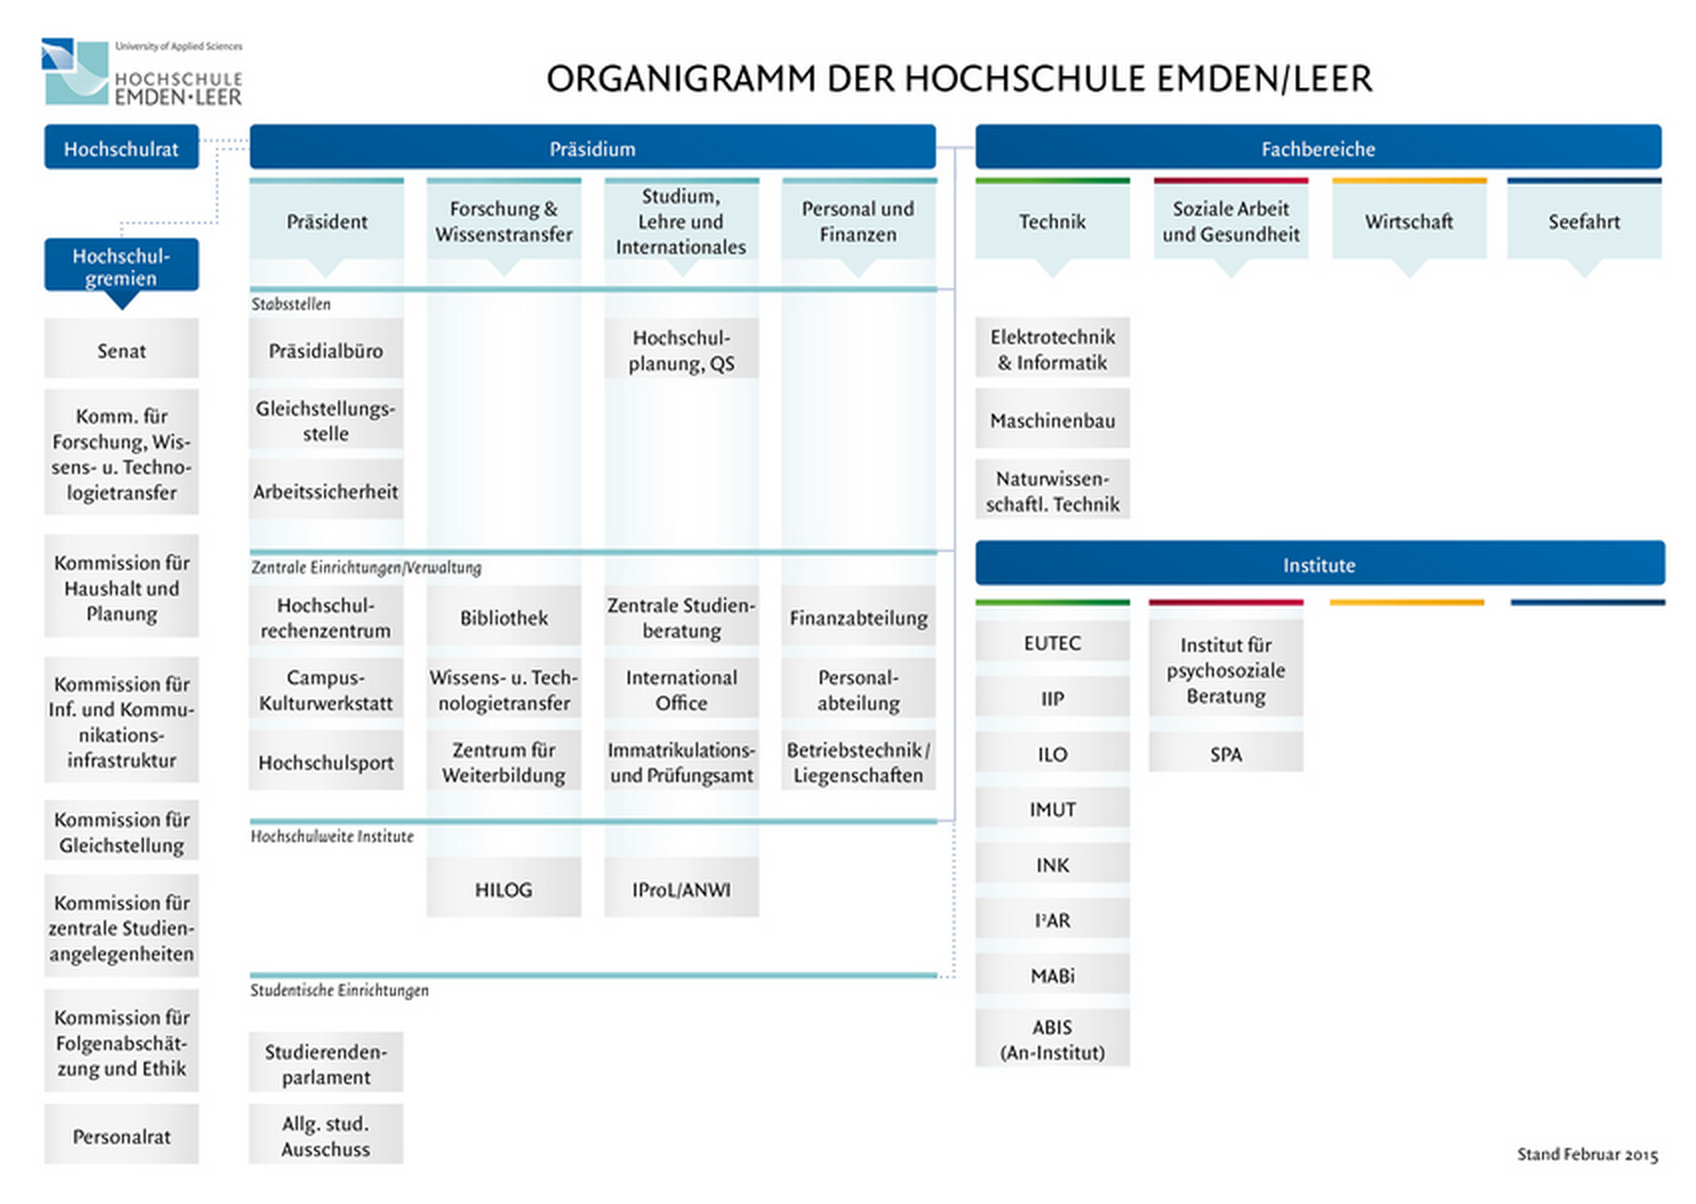
\includegraphics[width=15.501cm,height=11.003cm]{EntwurfKapitel2Gruppe220150528VW-img/EntwurfKapitel2Gruppe220150528VW-img005.png}
\caption[Organigramm der Hochschule Emden Leer]{Organigramm der Hochschule Emden Leer}

\end{figure}
\subsection[]{}
\subsection[2.3.1 Fachbereiche]{\bfseries 2.3.1 Fachbereiche}
{\sffamily\mdseries\color{black}
Die einzelnen Fachbereiche sind unter anderem durch die Mitgliedschaft in Arbeitsgruppen in den
Informationsbeschaffungsprozess involviert (siehe Kapitel 2.3.3). }


\bigskip

{\sffamily\mdseries\color{black}
Alle Fachbereiche verfügen über die Berechtigung relevante Informationen in dem Infosys darzustellen. Infosys ist eine
zentrale Plattform, welche online auf der Webseite der Hochschule Emden/Leer öffentlich von jedem eingesehen werden
kann oder vor Ort \ in den Eingangsbereichen der jeweiligen Fachbereiche über Dashboards. Es werden, nach Fachbereich
sortiert, die wichtigsten Neuigkeiten als Newsticker dargestellt und der Zugriff auf alle Vorlesungspläne der
Fachbereiche ist gegeben um so zügig auf organisatorische Inhalte zugreifen zu können. }


\bigskip

{\centering\sffamily\color[rgb]{0.77254903,0.0,0.043137256}
(PLATZHALER – Screenshot Info Sys)
\par}


\bigskip

{\sffamily\mdseries\color{black}
In den nachfolgenden Kapiteln wird nur auf die Besonderheiten der einzelnen Fachbereiche eingegangen.}

\subsubsection{2.3.1.1 Seefahrt}
{\sffamily\mdseries\color{black}
Bei dem Fachbereich Seefahrt handelt es sich um einen relativ kleinen Fachbereich. Seefahrt ist \ nur an dem Standort
Leer vertreten. Dieser Fachbereich verwendet kein zentrales System zur Vorlesung und Raumplanung, sondern eine
Eigenentwicklung.}

\subsubsection{2.3.1.2 Technik}
{\sffamily\mdseries\color{black}
Eine Besonderheit dieses Fachbereiches ist, dass für den Laborbetrieb ein Rechennetz neben dem zentralen Rechennetz der
Hochschule Emden/Leer betrieben wird. Da unter anderem der Bereich „IT-Sicherheit“ ein wichtiger Aspekt in dem
Studiengang Informatik ist, kommt es zu besonderen Konstellationen im Bereich der Forschung. Dieser Bereich verwaltet
sein Netz selbst und ist somit autark vom allgemeinen Hochschulrechennetz. }

\subsubsection[2.3.1.3 Wirtschaft ]{\itshape 2.3.1.3 Wirtschaft }
{\sffamily\itshape\color{black}
Wird ggf. gestrichen}

\subsubsection[2.3.1.4 Soziale Arbeit und Gesundheit]{\itshape 2.3.1.4 Soziale Arbeit und Gesundheit}
{\sffamily\itshape\color{black}
Wird ggf. gestrichen}

\subsection[2.2.3 Präsidium]{\bfseries 2.2.3 Präsidium}
{\sffamily\mdseries\color{black}
Das Präsidium insbesondere mit dem Bereich zentrale Verwaltung ist durch die Mitgliedschaft in Arbeitsgruppen in den
Informationsbeschaffungsprozess involviert. Eine besondere Stelle, im Bezug auf die Repräsentation von Informationen
besonders das Erscheinungsbild nach außen (siehe Kapitel 2.6), stellt eine Stabsstelle von dem Präsidium da. Das
Präsidialbüro ist unter anderem für den Bereich Hochschulmarketing zuständig.}

\subsection[2.3.2.2 Zentrale Verwaltung ]{\bfseries 2.3.2.2 Zentrale Verwaltung }
{\sffamily\mdseries\color{black}
(...)}

\subsubsection[2.3.2.3 Studentenverwaltung]{\itshape 2.3.2.3 Studentenverwaltung}
{\sffamily\itshape\color{black}
Wird ggf. gestrichen }

\subsubsection[2.3.2.4 Mitarbeiterverwaltung]{\itshape 2.3.2.4 Mitarbeiterverwaltung}
{\sffamily\itshape\color{black}
Wird ggf. gestrichen}

\subsubsection{2.3.2.5 Rechenzentrum }

\bigskip

{\sffamily\mdseries\color{black}
Das Hochschulrechenzentrum der Hochschule Emden/Leer ist stark in die Administration und Pflege der bestehenden Systeme
zur Informationsbereitstellung involviert. Neben der Administration von bestehenden Systemen obliegt dem
Hochschulrechenzentrum ebenfalls der Endkundensupport. }

\subsection[2.3.3 Arbeitsgruppen zum Informationsaustausch und zur Informationsbereitstellung]{\bfseries 2.3.3
Arbeitsgruppen zum Informationsaustausch und zur Informationsbereitstellung}
{\sffamily\mdseries\color{black}
Die Zuständigkeiten an der Hochschule, in Bezug auf Informationssammlung, Beschaffung und Aufbereitung von
Informationen, ist bereits durch Arbeitsgruppen in wichtigen Bereichen geregelt. Durch das Interview mit dem Leiter des
Hochschulrechenzentrums der Hochschule Emden/Leer konnte ein Einblick in die bestehenden Gremien geschaffen werden.
Derzeit existieren drei Arbeitsgruppen, welche für die Informationsverteilung in den jeweiligen Bereichen relevant
sind:}


\bigskip

\liststyleLii
\begin{itemize}
\item {\sffamily\color{black}
Zahlen, Daten und Fakten (ZDF)}
\item {\sffamily\color{black}
WEB}
\item {\sffamily\color{black}
Moodle}
\end{itemize}
\subsubsection{2.3.3.1 Zahlen, Daten und Fakten (ZDF)}
{\sffamily\mdseries\color{black}
ZDF setzt sich zusammen aus den Verwaltungsabteilungen Finanzen, Personal, Presse und Rechenzentrum. Dieses Gremium ist
zuständig für die Aufbereitung und zur Verfügung Stellung von Kennzahlen wie zum Beispiel aktuelle Kennzahlen zu
eingeschriebenen Studierenden pro Studiengang. \textbf{\textcolor[rgb]{0.9843137,0.0,0.02745098}{\ }}ZDF ist für einen
Unterbereich der offiziellen Webseite der Hochschule Emden/Leer zuständig. Die Kennzahlen und Zahlen werden
gruppenbasiert erstellt. Es werden grobe Kennzahlen erzeugt, welche öffentlich zugänglich sind und detailliertere
Zahlen für die Mitarbeiter, mit welchen sie arbeiten können. Dekane erhalten speziellere Zahlenwerte.}

\subsubsection[2.3.3.2 WEB]{2.3.3.2 WEB}
{\sffamily\mdseries\color{black}
Es existiert eine Arbeitsgruppe, welche für die Gestaltung und den Inhalt der öffentlichen Webseite der Hochschule
Emden/Leer verantwortlich ist. In dieser Arbeitsgruppe sind aus jedem Fachbereich Repräsentanten mit einbezogen.}

{\sffamily\mdseries\color{black}
Die Leitung des Web-Teams obliegt dem Präsidialbüro.
\footnote{\ http://www.hs-emden-leer.de/fileadmin/user\_upload/Einrichtungen/Praesidialbuero/Organigramm\_Praesidialbuero\_Juli2013\_01.pdf}}

\subsubsection{2.3.3.3 Moodle}
{\sffamily\mdseries\color{black}
In der Arbeitsgruppe „Moodle“ sind sowohl Repräsentanten aus jedem Fachbereich involviert sowie auch Repräsentanten aus
der Verwaltungsebene. Da das Moodle E-learning System mittlerweile als ein zentrales Moodle für alle Bereiche
eingeführt wurde, haben die Mitglieder aus den Fachbereichen unter anderem das Recht Kurse im Moodle freischalten zu
können. }


\bigskip

\section{2.4 Definierte und bestehende Prozesse (Reglung und Handhabung von vorhandenen Informationen)}
\subsection[2.4.1 Wissensmanagement]{\bfseries 2.4.1 Wissensmanagement}
{\sffamily\mdseries\color{black}
\textstyleAbsatzStandardschriftart{Wissensmanagement ist für die Hochschule Emden/Leer ein sehr wichtiger Aspekt, da Sie
täglich mit dem Erwerb, der Entwicklung, dem Transfer sowie der Nutzung von Wissen konfrontiert wird. Für den Betrieb
eines erfolgreichen Wissensmanagements ist an ein klares Regelwerk die Voraussetzung. \ }}

\subsection[2.4.2 E{}-learning]{\bfseries 2.4.2 E-learning}
{\sffamily\color{black}
Laut Michael Kerres ist E-Learning das Lehren und Lernen bei dem elektronische Medien für die Präsentation und
Distribution von Lehrmaterialien und Kommunikation zum Einsatz kommen. }

\subsubsection[2.4.2.1 E{}-Learning an der Hochschule Emden/Leer]{2.4.2.1 E-Learning an der Hochschule Emden/Leer}
{\sffamily\color{black}
E-Learning ist an der Hochschule Emden/Leer ein sehr wichtiges Thema, da an der Hochschule der Studiengang
Medieninformatik (Online), Wirtschaftsinformatik (Online) akkreditiert \ wurde. Nun soll dargelegt werden ob in den
Präsenzstudiengängen ebenfalls das Thema E-Learning Einzug gehalten hat.}

\subsubsection{2.4.2.2 E-Learning in den Präsenzstudiengängen}
{\sffamily\mdseries\color{black}
Es soll betrachtet werden in welchen Präsenzstudiengängen E-Learning eingesetzt wird.}


\bigskip

{\centering\sffamily\color{black}
\textstyleAbsatzStandardschriftart{\textbf{\textcolor{red}{(PLATZHALTER GRAFIK)}}}
\par}


\bigskip

{\sffamily\mdseries\color{black}
Aus der Grafik geht hervor, dass der Fachbereich SAG (Soziale Arbeit und Gesundheit) der Vorreiter aller Fachbereiche
mit der Einführung eines E-Learning Systems war. SAG setzt mehr als 200 Onlinekurse im Präsenzstudium ein. Auch für die
Anmeldung an verschiedenen Kursen kommt ein Online-System zum Einsatz.}


\bigskip

{\sffamily\mdseries\color{black}
\textstyleAbsatzStandardschriftart{Es folgt dann der Fachbereich Technik in dem E-Learning ebenfalls sehr stark
verbreitet ist, da die Studiengänge Medieninformatik und Wirtschaftsinformatik als reine Onlinestudiengänge in diesem
etabliert sind.}}


\bigskip

{\sffamily\mdseries\color{black}
Weniger stark wird E-Learning vom Fachbereich Wirtschaft betrieben. Das geringste Nutzungsverhalten ist im Fachbereich
Seefahrt zu verzeichnen.}


\bigskip

{\sffamily\color{black}
Trotz des unterschiedlichen Nutzungsverhaltens hat E-Learning in allen Fachbereich Einzug gehalten.}

\subsubsection{2.4.2.3 Einsatz von E-Learning-Anwendungen in den Präsenzstudiengängen}
{\sffamily\mdseries\color{black}
Im diesem Abschnitt wird erläutert, ob die Anwendungen Adobe Connect, Moodle im Präsenzstudiengang eingesetzt werden.}

\subsubsection[2.4.2.3.1 Adobe Connect]{2.4.2.3.1 Adobe Connect}
{\sffamily\mdseries\color{black}
Adobe Connect ist eine Kommunikationsplattform zur Bereitstellung von Webmeetings und E-Learning-Inhalten.}


\bigskip

{\sffamily\mdseries\color{black}
Ausschließlich der Fachbereich Technik (E+I) nutzt durch seine Onlinestudiengänge die Plattform Adobe Connect als Medium
des visuellen Austausches von Bild und Sprache. In den Präsenzstudiengängen kommt die Plattform nicht zum Einsatz, da
der persönliche Austausch von Studierenden und Dozenten in den täglichen Präsenzen stattfindet.}

\subsubsection{2.4.2.3.2 Moodle}
{\sffamily\mdseries\color{black}
Die Hochschule Emden/Leer setzt Moodle als Lernplattform ein. Moodle ist ein freies objektorientiertes
Kursmanagementsystem welches prädestiniert ist für den Einsatz von E-Learning
Inhalten.\footnote{\url{https://moodle.hs-emden-leer.de/moodle/}}}


\bigskip

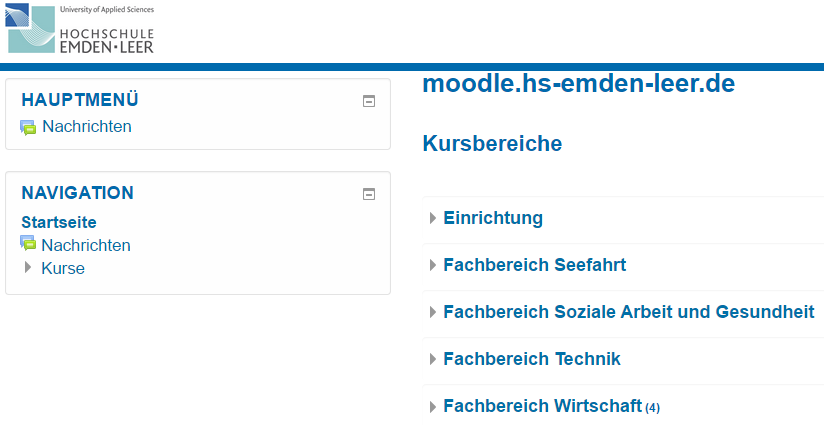
\includegraphics[width=15.501cm,height=7.994cm]{EntwurfKapitel2Gruppe220150528VW-img/EntwurfKapitel2Gruppe220150528VW-img006.png}
\captionof{figure}[Übersicht Moodle für alle]{Übersicht Moodle für alle}


{\sffamily\color{black}
Durch den Einsatz von Moodle in allen Fachbereichen, wird das volle Leistungsspektrum des Systems ausgenutzt. Folgende
Funktionalitäten werden angeboten:}


\bigskip

\liststyleLiii
\begin{itemize}
\item {\sffamily\color{black}
\textstyleAbsatzStandardschriftart{Lernvideos}}
\item {\sffamily\color{black}
\textstyleAbsatzStandardschriftart{Vorlesungsskripte}}
\item {\sffamily\color{black}
\textstyleAbsatzStandardschriftart{Forum}}
\item {\sffamily\color{black}
\textstyleAbsatzStandardschriftart{Kalender}}
\item {\sffamily\color{black}
\textstyleAbsatzStandardschriftart{Mail-Connect}}
\end{itemize}
{\sffamily\mdseries\color{black}
\textstyleAbsatzStandardschriftart{Für jeden Fachbereich wird der volle Funktionsumfang der Plattform zur Verfügung
gestellt, auch wenn nicht jeder Fachbereich jeden Service nutzt. }}


\bigskip

\subsubsection{2.4.2.4 Zentrale Informationsbereitstellung durch Datenlaufwerke}
{\sffamily\mdseries\color{black}
Für alle beteiligten der Hochschule Emden/Leer werden spezielle Datenlaufwerke zur Verfügung gestellt. Es handelt sich
um 3 Netzlaufwerke auf den Fileservern der Hochschule.\footnote{\url{https://connect.hs-emden-leer.de/cgi-bin/portal}}}

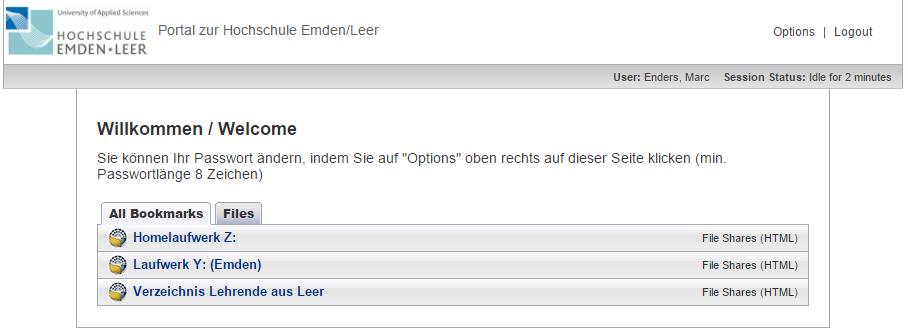
\includegraphics[width=15.501cm,height=5.667cm]{EntwurfKapitel2Gruppe220150528VW-img/EntwurfKapitel2Gruppe220150528VW-img007.png}
\captionof{figure}[Zugriff auf die Datenlaufwerke von extern]{Zugriff auf die Datenlaufwerke von extern}


{\sffamily\bfseries\color{black}
2.4.2.4.1 Laufwerk Z}

{\sffamily\mdseries\color{black}
\textstyleAbsatzStandardschriftart{Auf dem Laufwerk Z befinden sich die Daten des Home-Verzeichnisses jedes einzelnen
Benutzers. Meldet sich dieser an beliebigen Rechnern des Rechnerpools an, werden die Inhalte Ihres Home-Verzeichnisses
automatisch\textcolor[rgb]{0.4392157,0.1882353,0.627451}{ }eingebunden. Der interne Zugriff auf die eigenen Dateien ist
von jedem Rechner des Pools möglich, da servergespeicherte Profile zum Einsatz kommen. Auch von externe können die
Studierenden problemlos auf die Ressourcen der Datenlaufwerke zugreifen.}}


\bigskip

{\sffamily\bfseries\color{black}
2.4.2.4.2 Laufwerk Y}

{\sffamily\mdseries\color{black}
\textstyleAbsatzStandardschriftart{Für den gemeinsamen Austausch der Daten wurde das Transferlaufwerk Y eingerichtet.
Hier werden zentral Ressourcen für alle Studierenden und Lehrenden aus Emden zum Austausch zur Verfügung gestellt.}}

\subsubsection{2.4.2.4.3 Verzeichnis Lehrende aus Leer}
{\sffamily\mdseries\color{black}
\textstyleAbsatzStandardschriftart{Zusätzlich zum Transferlaufwerk steht das Verzeichnis der Lehrenden aus Leer \ zur
Verfügung. Hier stellen die Lehrenden Inhalte zur Verfügung.}}

\subsubsection[2.4.2.5 Moodle vs. Datenlaufwerke für Präsenzstudenten]{2.4.2.5 Moodle vs. Datenlaufwerke für
Präsenzstudenten}
{\sffamily\mdseries\color{black}
An der Moodle-Plattform melden sich die Nutzer über eine webbasierte Oberfläche am System an. Um Dateien zur Verfügung
zu stellen, muss auf der Weboberfläche zu den gewünschten Reitern navigiert werden.}


\bigskip

{\sffamily\color{black}
\textstyleAbsatzStandardschriftart{Stellt man die Datenlaufwerke (Y Laufwerk und Transferlaufwerk der Lehrenden) der
Moodle-Plattform gegenüber \ und betrachtet nur den Aspekt des Datenaustausches, so wird deutlich, dass der
Dateiaustausch über \ \ Datenlaufwerke in Bezug auf Komfort und Aufwand deutlich besser für die Präsenzstudierenden
geeignet ist, als die Dateiablage über die Moodle-Plattform. Die über die Datenlaufwerke zur Verfügung gestellten
Inhalte können von den Studierenden mit wenig Aufwand intuitiv erreicht werden.}}


\bigskip

{\sffamily\color{black}
\textstyleAbsatzStandardschriftart{Aus dem Interview mit dem Rechenzentrumsleiter Herrn Günter Müller kristallisierte
sich heraus, dass der Fachbereich Wirtschaft die Datenlaufwerke am stärksten und der Fachbereich Technik und andere
Fachbereiche diese weniger stark nutzen.}}

\subsection[2.4.4 Sicherheitsaspekte]{\bfseries 2.4.4 Sicherheitsaspekte}
{\sffamily\bfseries\color{black}
(...)}

\subsubsection{2.4.4.1 Sicherheitsrichtlinien an der Hochschule Emden / Leer}
{\sffamily\mdseries\color{black}
Der Einsatz von Sicherheitsrichtlinien ist ein wichtiges Thema an Hochschulen. Sicherheitsrichtlinien beschreiben die
Sicherstellung von Verfügbarkeit, Integrität, Vertraulichkeit und Authentizität von Informationen.}

{\sffamily\mdseries\color{black}
\textstyleAbsatzStandardschriftart{An der Hochschule Emden/Leer werden als Basis für die Informationssicherheit Teile
des IT-Grundschutz-Kataloges umgesetzt. Nicht alle Empfehlungen des BSI sind an einer kleinen Hochschule, wie die
Hochschule Emden/Leer es ist, \ umsetzbar.}}

{\sffamily\mdseries\color{black}
An den Serverräumen der Hochschule ist die Umsetzung der IT-Grundschutzmaßnahmen deutlich zu erkennen.}

{\sffamily\mdseries\color{black}
Folgende physikalische Schutzmaßnahmen wurden an der Hochschule Emden/Leer in den Serverräumen umgesetzt:}


\bigskip

\liststyleLiv
\begin{itemize}
\item {\sffamily\color{black}
einbruchsicher}
\item {\sffamily\color{black}
feuergemeldet}
\item {\sffamily\color{black}
videoüberwacht}
\item {\sffamily\color{black}
Lage der Serverräume im 1 OG (Wasserschutz)}
\end{itemize}
\subsubsection[2.4.4.2 Einsatz von ITIL]{\textstyleAbsatzStandardschriftart{2.4.4.2 Einsatz von ITIL}}
{\sffamily\mdseries\color{black}
Die IT Infrastructure Libary (ITIL) ist eine Sammlung von Best Practises zur Umsetzung eines IT-Service-Managements
(ITSM). In diesem Regelwerk werden die für den Betrieb einer IT-Infrastruktur notwendigen Prozesse und Werkzeuge
beschrieben.}

{\sffamily\color{black}
\textstyleAbsatzStandardschriftart{Der ITIL-Prozess ist an der Hochschule Emden/ Leer nicht etabliert, da die
Personaldecke für die Umsetzung eines 1st und 2nd-Level Supports nicht gegeben
ist.}\footnote{\url{http://de.wikipedia.org/wiki/IT_Infrastructure_Library}}}

\subsubsection[2.4.4.3 Umsetzung von ISO/IEC 27001]{\textstyleAbsatzStandardschriftart{2.4.4.3 Umsetzung von ISO/IEC
27001}}
{\sffamily\mdseries\color{black}
Die ISO/IEC 27001 Zertifizierung wird auf Basis des IT-Grundschutzes vergeben. Durch die Zertifizierung des ISO/IEC
27001 Standards haben Unternehmen, Behörden, Organisationen die Möglichkeit, ihre Bemühungen um Informationssicherheit
nach innen und außen zu dokumentieren.}


\bigskip

{\sffamily\mdseries\color{black}
Das Einsatzszenario ist an der Hochschule Emden/Leer nicht gegeben, da für Umsetzung die Personaldichte zu gering ist.
Für die Erfüllung der Zertifizierung würde riesiger Personaloverhead
entstehen.\footnote{\href{https://www.bsi.bund.de/DE/Themen/ZertifizierungundAnerkennung/Zertifizierung27001/GS_Zertifizierung_node.html}{\textstyleHyperlink{https://www.bsi.bund.de/DE/Themen/ZertifizierungundAnerkennung/Zertifizierung27001/GS\_Zertifizierung\_node.htm}}\href{https://www.bsi.bund.de/DE/Themen/ZertifizierungundAnerkennung/Zertifizierung27001/GS_Zertifizierung_node.html}{\textstyleHyperlink{l}}}}


\bigskip

{\sffamily\bfseries\color{black}
2.4.4.4 Single Sign-on}

{\sffamily\bfseries\color{black}
(...)}

{\sffamily\bfseries\color{black}
2.4.4.5 Fazit Sicherheitsrichtlinien}

{\sffamily\mdseries\color{black}
\textstyleAbsatzStandardschriftart{Abschließend ist zu sagen, dass an der Hochschule Emden/Leer der IT-Sicherheitsaspekt
ein sehr wichtiges Thema ist. Als kleine Hochschule ist es auf Grund der Personaldichte nicht möglich, alle
Empfehlungen des BSI-Grundschutzes, ITIL und ISO/IEC 27001 umzusetzen. Jedoch sucht sich die Hochschule aus den
Regelwerken die Empfehlungen heraus, die auf Grund der Personaldichte umsetzbar sind. \ Dies bildet eine sehr gute
Basis im Hinblick auf das sehr anspruchsvolle Thema IT-Sicherheit.}}

\section{2.5 Repräsentation von Informationen}
{\sffamily\mdseries\color{black}
Ein wichtiger Aspekt bei der Hochschule ist die Repräsentation von Informationen. Hier spielt sowohl das
Erscheinungsbild nach außen sowie die Repräsentation von Informationen innerhalb der einzelnen Bereiche eine
essenzielle Rolle. }

\subsection[2.5.1 Erscheinungsbild nach außen]{\bfseries 2.5.1 Erscheinungsbild nach außen}
{\sffamily\mdseries\color{black}
(...)}

\subsection[2.5.2 Studentengewinnung]{\bfseries\color{black} 2.5.2 Studentengewinnung}
{\sffamily\mdseries\color{black}
Wie in Kapitel 2.3 bereits erwähnt obliegt die Zuständigkeit der des Marketings dem Präsidialbüro. Generell ist die
Studentengewinnung wie folgt aufgeteilt: \ Zum einen existiert eine zentrale Studienberatung, bei welcher sich
Interessenten direkt informieren können und zum anderen werden regelmäßig Besuche der Hochschule bei Schulen in der
Region durchgeführt. Mitglieder der jeweiligen Fachbereiche berichten vor Ort in der jeweiligen Schule über die
Möglichkeiten. Neben diesen beiden ...verfügt die Hochschule Emden/Leer auch über diverse Online Medien bei welchen
sich Interessenten informieren können. }

\subsection[2.5.3 Corporate Identity]{\bfseries 2.5.3 Corporate Identity}
{\sffamily\mdseries\color{black}
Die Hochschule verfügt über eine Corporate Design (CD) Reglung, welche auf der Webseite öffentlich eingesehen werden
kann. Diese wird von dem Bereich Marketing zur Verfügung gestellt und gepflegt.
\footnote{http://www.hs-emden-leer.de/einrichtungen/praesidialbueropresse-und-oeffentlichkeitsarbeit/corporate-design.html}
}

{\sffamily\mdseries\color{black}
Diese Reglung umfasst unter anderem einen CD
Regelungsguide\footnote{http://www.hs-emden-leer.de/fileadmin/user\_upload/Einrichtungen/Praesidialbuero/Downloads/HS\_CD\_Manual\_08\_2013.pdf},
sowie diverse Vorlagen für Power Point Präsentationen bis hin zum allgemeinen Logo und Logos für jeden Fachbereich.}



\begin{figure}
\centering

\includegraphics[width=8.58cm,height=3.039cm]{EntwurfKapitel2Gruppe220150528VW-img/EntwurfKapitel2Gruppe220150528VW-img008.png}
\caption[Allgemeines Logo der Hochschule Emden/Leer]{Allgemeines Logo der Hochschule Emden/Leer}

\end{figure}
\begin{figure}
\centering

\includegraphics[width=8.576cm,height=3.044cm]{EntwurfKapitel2Gruppe220150528VW-img/EntwurfKapitel2Gruppe220150528VW-img009.png}
\caption[Logo des Fachbereiches Technik]{Logo des Fachbereiches Technik}

\end{figure}
\subsection[2.5.4 Handling von Bewerberdaten]{\bfseries 2.5.4 Handling von Bewerberdaten}
{\sffamily\mdseries\color{black}
Durch das Interview mit Herrn Günter Müller konnte festgestellt werden, wie das allgemeine Handling von Bewerberdaten
aus Sicht des Rechenzentrums stattfindet. }

{\sffamily\mdseries\color{black}
Der Bewerber meldet sich an dem HIS der Hochschule mit seinen Daten an und dieser Account ist nur für die Dauer des
Bewerbungszeitraumes aktiv. Wird der Bewerber nicht angenommen, so wird dieser Account im Anschluss wieder gelöscht.
Wird der Bewerber jedoch akzeptiert, wird der vorhandene temporäre Account in einen permanenten Account mit erweiterten
Informationseingaben, wie z.B. Krankenkassendaten, umgewandelt. Auf diese Weise ist sichergestellt, das nur aktive
Studenten einen Account zur Verfügung gestellt bekommen. }

\section{2.6 Kooperations-Situation mit anderen Hochschulen}
{\sffamily\mdseries\color{black}
Kooperationsverhältnisse mit anderen Hochschulen, Verbänden und Unternehmen spielt auch an der Hochschule Emden/Leer
eine sehr entscheidende Rolle, da durch die Kooperation verschiedene Services zur Verfügung stehen.}

\subsection[2.6.1 Regionaler Bezug zu Hochschulen (Mitgliedschaften)]{\bfseries 2.6.1 Regionaler Bezug zu Hochschulen
(Mitgliedschaften)}
{\sffamily\mdseries\color{black}
Die Hochschule Emden/Leer pflegt ein enges Kooperationsverhältnis mit dem Jade-Hochschulverbund. Über das Lokale
Bibliothekssystem Ostfriesland/Wilhelmshaven (LBS) wird auf die gemeinsamen \ Bibliotheksbestände
zugegriffen.\footnote{\textstyleHyperlink{\ }http://www.jade-hs.de/service-verwaltung/hochschulbibliothek/bestand/online-kataloge/}}


\bigskip

{\sffamily\mdseries\color{black}
Durch ein gemeinsames Promotionskolleg findet ebenfalls eine intensive Zusammenarbeit mit der Universität Vechta statt.
Aktuell baut die Hochschule Emden/Leer die Kooperation zur Hochschule Osnabrück
aus.\footnote{\textstyleHyperlink{\ }\href{http://www.hs-emden-leer.de/hochschule/profil.html}{http://www.hs-emden-leer.de/hochsc}hule/profil.html}}


\bigskip

{\sffamily\mdseries\color{black}
Der Rechenzentrumsleiter Herr Günter Müller ist selbst Mitglied des Arbeitskreises LANIT / HRZ. Hier treffen die Leiter
der Rechenzentren Niedersachsens aufeinander und tauschen Ihre Erfahrungen aus. Der Arbeitskreis befasst sich mit
Themen der IT-Infrastruktur für Forschung, Lehre und Verwaltung an den Hochschulen Niedersachsens. Zu Schwerpunktthemen
wurden Arbeitsgruppen eingerichtet. \ Ebenfalls werden hochschulübergreifend Projekte
durchgeführt.\footnote{\textstyleHyperlink{\ }http://www.lanit-hrz.de/}}


\bigskip

{\sffamily\mdseries\color{black}
Das ZKI (Zentren für Kommunikation und Informationsverarbeitung in Lehre und Forschung e.V.) spielt für die Hochschule
eine wichtige Rolle. Ziel dieses Vereins ist es, die Kooperation zwischen den ZKI/Rechenzentren, Meinungs- und
Erfahrungsaustausch, sowie die Beratung und Zusammenarbeit mit bildungs- und wirtschaftsfördernden Einrichtungen zu
fördern. In den immer wiederkehrenden Tagungen erarbeitet der Arbeitskreis Lösungsvorschläge für aktuelle Probleme der
Informationsverarbeitung. Aktuelle Themen sind z.B. eine Studie über das Thema: „CIOs und IT-Governance an deutschen
Hochschulen“. \footnote{\textstyleHyperlink{\ }https://www.zki.de/zki-nachrichten/einzelbeitrag/1215/}}


\bigskip

{\sffamily\mdseries\color{black}
Durch den Verein DFN (Deutsches Forschungsnetz) wird der Hochschule eine Vielzahl von maßgeschneiderten
Kommunikationsanwendungen (DFN-Diensten) zur Verfügung gestellt. Der DFN-Verein ist ein von der Wissenschaft selbst
organisiertes Kommunikationsnetz für Wissenschaft und Forschung in Deutschland. Er verbindet Hochschulen und
Forschungseinrichtungen miteinander und ist in den europäischen und weltweiten \ Verbund der Forschungsnetze
integriert.\footnote{\textstyleHyperlink{\textcolor{black}{\ }}https://www.dfn.de/}}

\subsection[2.6.2 Kooperation zwischen Unternehmen]{\bfseries 2.6.2 Kooperation zwischen Unternehmen}
{\sffamily\mdseries\color{black}
Regional betrachtet arbeitet die Hochschule Emden/Leer mit 82\% der Unternehmen der Region zusammen. Der Vorteil dieser
Kooperation ist es, dass zum einen die Studierenden die Möglichkeit haben ihre Fähigkeiten in der Praxis anzuwenden und
zum anderen können die Unternehmen das Know-How \ der Hochschule nutzen und sinnvoll einsetzen. Der Wissenstransfer der
in der Hochschule erfolgt, bietet den Unternehmen einen erheblichen
Mehrwert.\footnote{\ \href{http://www.hs-emden-leer.de/en/news-events/news/article/hochschule-weit-vorn-bei-kooperation-mit-unternehmen.html}{http://www.hs-emden-leer.de/en/news-events/news/article/hochschule-weit-vorn-}\textcolor{black}{bei}{}-kooperation-mit-unternehmen.html}}

\subsection[2.6.3 Eingesetzte IT{}-Systeme durch Mitgliedschaft im DFN{}-Verein]{\bfseries\color{black} 2.6.3
Eingesetzte IT-Systeme durch Mitgliedschaft im DFN-Verein}
{\sffamily\mdseries\color{black}
Die angebotenen Dienste des Deutsches Forschungsnetzes sind für den Zweck von Wissenschaft und Forschung maßgeschneidert
worden. Ein besonderes Augenmerk liegt hier auf die gute Integration der Dienste in der Prozesse der Hochschulen. \ Auf
die Dienste die der DFN-Verein der Hochschule Emden/Leer zur Verfügung stellt, wird fort folgend nun näher
eingegangen.\footnote{\url{https://www.dfn.de/dienstleistungen/}}}

\subsubsection[2.6.3.1 DFNRoaming/eduroam]{\bfseries\color{black} 2.6.3.1 DFNRoaming/eduroam}

\bigskip

{\sffamily\mdseries\color{black}
Die Hochschule Emden/Leer ist Mitglied des deutschen Forschungsnetzes (DFN). Durch diese Kooperation nutzt die
Hochschule den durch das DFN zur Verfügung gestellten Dienst DFNRoaming/eduroam. Dieser ermöglich es, registrierten
Nutzern über dienstkonforme WLANs Zugang zum Wissenschaftsnetz zur Verfügung zu stellen. \ Der DFN-Verein betreibt und
pflegt die eduroam Förderationsserver in
Deutschland.\footnote{\href{https://www.dfn.de/dienstleistungen/dfnroaming/}{\textstyleHyperlink{https://www.dfn.de/dienstleistungen/dfnroaming}}\textstyleHyperlink{/}}}

{\sffamily\color{black}
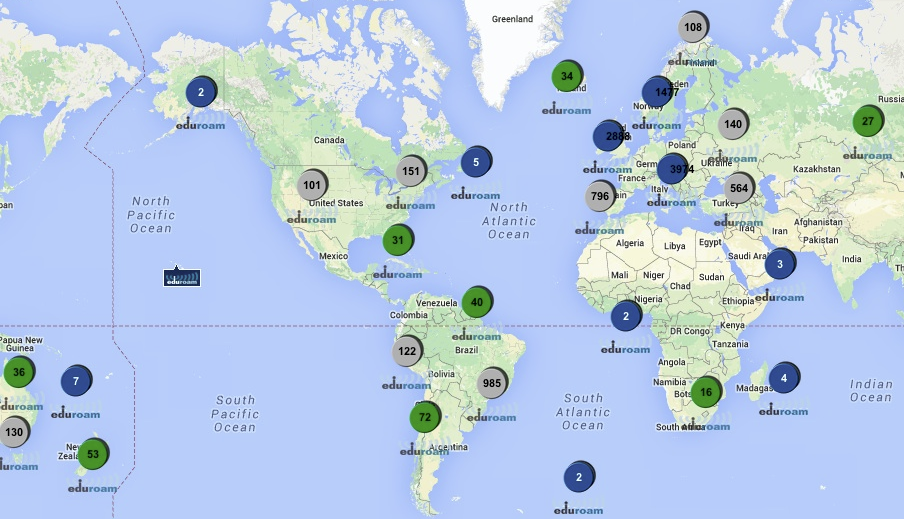
\includegraphics[width=15.501cm,height=8.95cm]{EntwurfKapitel2Gruppe220150528VW-img/EntwurfKapitel2Gruppe220150528VW-img010.png}
\captionof{figure}[http://weill.cornell.edu/its/images/eduroam{}-map.jpg]{http://weill.cornell.edu/its/images/eduroam-map.jpg}
\textbf{2.6.3.2 GigaMove der RWTH Aachen}}


\bigskip

{\sffamily\mdseries\color{black}
\textstyleAbsatzStandardschriftart{Die Rheinisch-Westfälische Technische Hochschule Aachen (RWTH Aachen) stellt eine
einfach zu nutzende Möglichkeit \ zum kurzfristigen Austausch großer Dateien zur Verfügung. Der Datenaustausch kann aus
zwei Richtungen angestoßen werden. Zum einen kann ein Nutzer eine Datei hochladen und die Anwendung erzeugt einen Link
zum Download, zum anderen kann eine Datei angefordert werden bei der die Anwendung einen Link generiert, der zu einem
Formular zum Upload der Datei führt. Jeder Nutzer darf standardmäßig Dateien in der Gesamtgröße von 10 GB für einen
Zeitraum von 14 Tagen auf den gehosteten Servern abspeichern. Der von der RWTH Aachen gehostete Dienst GigaMove wird
den Nutzern der Hochschule Emden/Leer zur Verfügung gestellt.}}


\bigskip

{\sffamily\color{black}
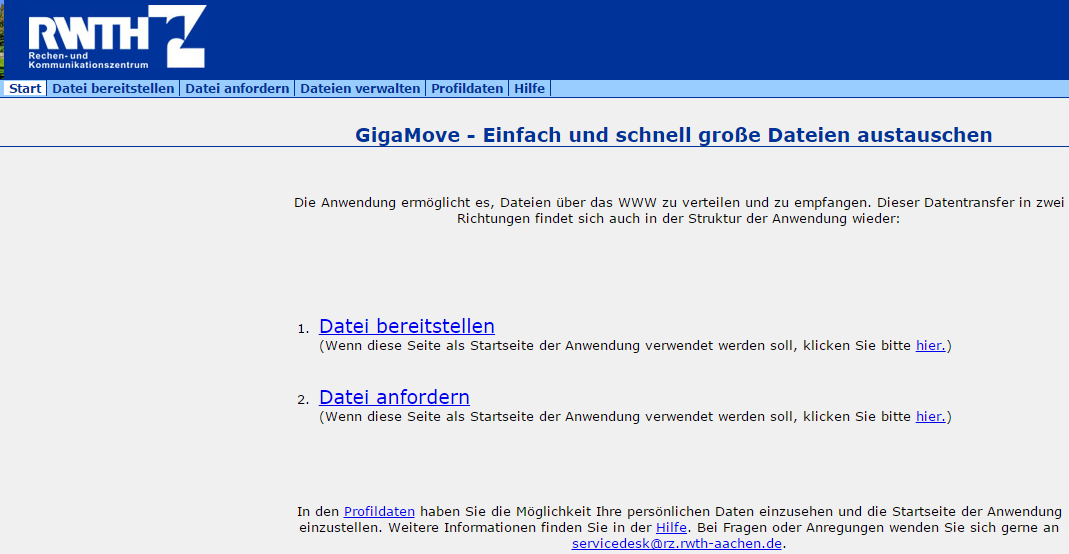
\includegraphics[width=15.501cm,height=8.033cm]{EntwurfKapitel2Gruppe220150528VW-img/EntwurfKapitel2Gruppe220150528VW-img011.png}
\captionof{figure}[https://gigamove.rz.rwth{}-aachen.de/instructions/wicket:pageMapName/wicket{}-0]{https://gigamove.rz.rwth-aachen.de/instructions/wicket:pageMapName/wicket-0}
\textbf{2.6.3.3 DFNVideoConference (DFNVC)}}


\bigskip

{\sffamily\mdseries\color{black}
\textstyleAbsatzStandardschriftart{DFVNC bietet den Nutzern die Möglichkeit von einem PC, einem Raumsystem oder einem
Telefon durch Nutzung des Wissenschaftsnetzes X-WiN mit einem oder mehreren Nutzern zu kommunizieren. Die Kommunikation
findet multimedial statt. Das Wissenschaftsnetz X-WiN ist die technische Plattform des deutschen
}\textstyleAbsatzStandardschriftart{Forschungsnetzes. Über das X-WiN sind die Hochschulen und Forschungseinrichtungen
in Deutschland untereinander und mit den Wissenschaftsnetzen in Europa auf anderen Kontinenten
vernetzt.}\footnote{\textstyleHyperlink{\ }https://www.dfn.de/dienstleistungen/dfnvc/}\textstyleAbsatzStandardschriftart{
An der Hochschule wird dieser Dienst ebenfalls genutzt.}}

\subsection[2.6.4 Authentifizierung über das Shibboleth{}-Verfahren]{\bfseries\color{black} 2.6.4 Authentifizierung über
das Shibboleth-Verfahren}
{\sffamily\color{black}
Das von der Hochschule eingesetzte Shibboleth-Verfahren ermöglicht den Studierenden und Mitarbeitern Ressourcen der
Anbieter SpringerLink, WISO, video2brain und andere Dienste nutzen. Hierbei muss \ bei der Anmeldung die Hochschule als
Heimatinstitution und die Hochschulkennung angegeben
werden.\footnote{\url{http://www.hs-emden-leer.de/no_cache/einrichtungen/bibliothek/medienangebot/elektronische-angebote/vpn-shibboleth.html}}}

\subsubsection[2.6.4.1 Springer Link]{\bfseries\color{black} 2.6.4.1 Springer Link}
{\sffamily\mdseries\color{black}
Studierende und Mitarbeiter der Hochschule Emden/Leer haben über die Springerlink-Kooperation Zugriff auf über 40.000
Bücher, 5 Millionen Artikel, 2200 Zeitschriften und 165 Nachschlagewerke. Des Weiteren kann jedes Dokument als *.pdf
heruntergeladen werden.\footnote{\ \url{http://link.springer.com/athens-shibboleth-login?previousUrl=\%2F}}}


\bigskip


\includegraphics[width=15.476cm,height=4.152cm]{EntwurfKapitel2Gruppe220150528VW-img/EntwurfKapitel2Gruppe220150528VW-img012.png}
\captionof{figure}[SpringerLink Startseite]{SpringerLink Startseite}


{\sffamily\bfseries\color{black}
2.6.4.2 WISO}

{\sffamily\mdseries\color{black}
Durch das Kooperationsverhältnis mit der GBI-Genios Deutsche Wirtschaftsdatenbank GmbH können die Mitglieder der
Hochschule Emden/Leer das komplette Angebot an Fachinformationen zu den Wirtschafts- und Sozialwissenschaften, zu
technischen Studiengängen und zur Psychologie \ nutzen. WISO bietet über 14 Mio. Literaturnachweise, 2100 elektronische
Bücher, 130 Mio. Artikel, 700.000 Marktdaten.\footnote{\ https://www.wiso-net.de/popup/ueber\_wiso}}

\subsubsection{2.6.4.3 video2brain}
{\sffamily\mdseries\color{black}
\textstyleAbsatzStandardschriftart{Seit 2015 ist für alle Mitarbeiter und Studierende der Zugang zum
Videostreaming-Portal der video2brain GmbH möglich. Schwerpunkt sind IT- und Kreativ-Themen, Lehrvideos für Fotografen,
Grafiker, Web- und Screendesigner. Das Verlagsangebot umfasst mehr als 1700
Video-Trainingskurse.}\footnote{http://de.wikipedia.org/wiki/Video2brain}}

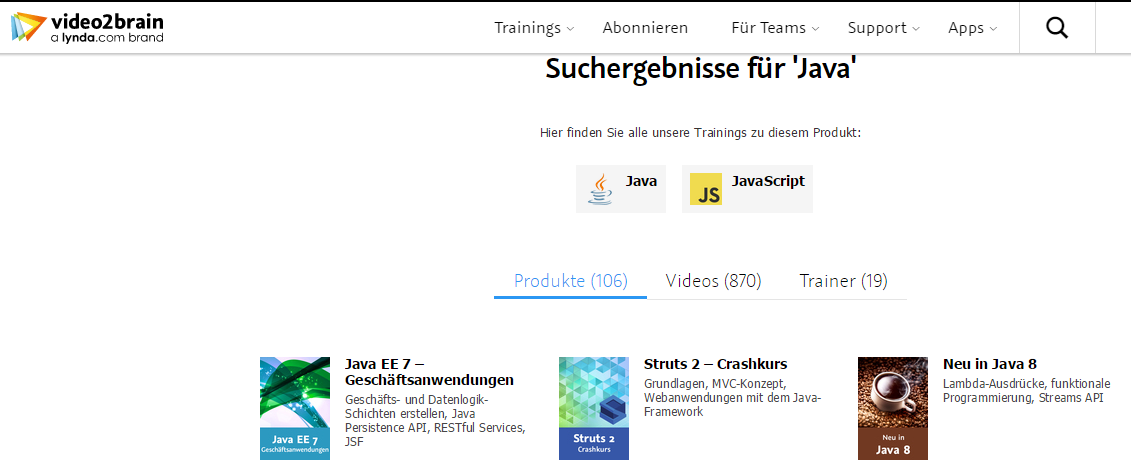
\includegraphics[width=15.501cm,height=6.482cm]{EntwurfKapitel2Gruppe220150528VW-img/EntwurfKapitel2Gruppe220150528VW-img013.png}
\captionof{figure}[Suchergebnisse für Java bei video2brain
(https://www.video2brain.com/de/search.htm?search\_entry=Java)]{Suchergebnisse für Java bei video2brain
(https://www.video2brain.com/de/search.htm?search\_entry=Java)}



\bigskip

{\sffamily\bfseries\color{black}
2.6.5 Support der Dienste}


\bigskip

{\sffamily\mdseries\color{black}
Für die zentral angebotenen Dienste eduroam, Shibboleth, GigaMove übernimmt die Hochschule Emden/Leer den
Endkundensupport. Die Mitarbeiter der Hochschule Emden/Leer bilden somit die zentrale Support-Schnittstelle und
delegieren Anfragen, die vor Ort nicht gelöst werden können, an die entsprechenden Anbieter weiter.}


\bigskip

{\sffamily\mdseries\color{black}
Diese Informationen teile uns der Leiter des Hochschulrechenzentrums Emden/Leer, Herr Günter Müller in dem
durchgeführten Interview mit.}

\section{2.7 Bewertung \& Gewichtung}
{\sffamily\mdseries\color{black}
Abschließend kann gesagt werden, dass die Hochschule Emden/Leer derzeit über kein Informationsmanagement verfügt. Es
werden Informationen zentral gesammelt und zentrale Systeme wie das Y-Laufwerk und die E-Learning Plattform Moodle
werden in allen Fachbereichen und in Teilen der Verwaltung eingesetzt.}

{\sffamily\mdseries\color{black}
Durch den starken Kooperationsverbund werden diverse Dienste, wie SpringerLink, WISO und video2brain bereits zentral zur
Verfügung gestellt (siehe Kapitel 2.6) \ und somit ist ein Teil des Wissensmanagements bereits gegeben. (...)}


\bigskip


\bigskip


\bigskip


\bigskip
\end{document}
